\documentclass[tikz,border=2pt]{standalone}
\usepackage{amsmath,amssymb}
\usepackage{tikz}
\usetikzlibrary{arrows.meta}

\begin{document}
% S_3: the 3! = 6 permutations of {1,2,3}, pictured as the symmetries of a labelled triangle:
% three rotations and three reflections.
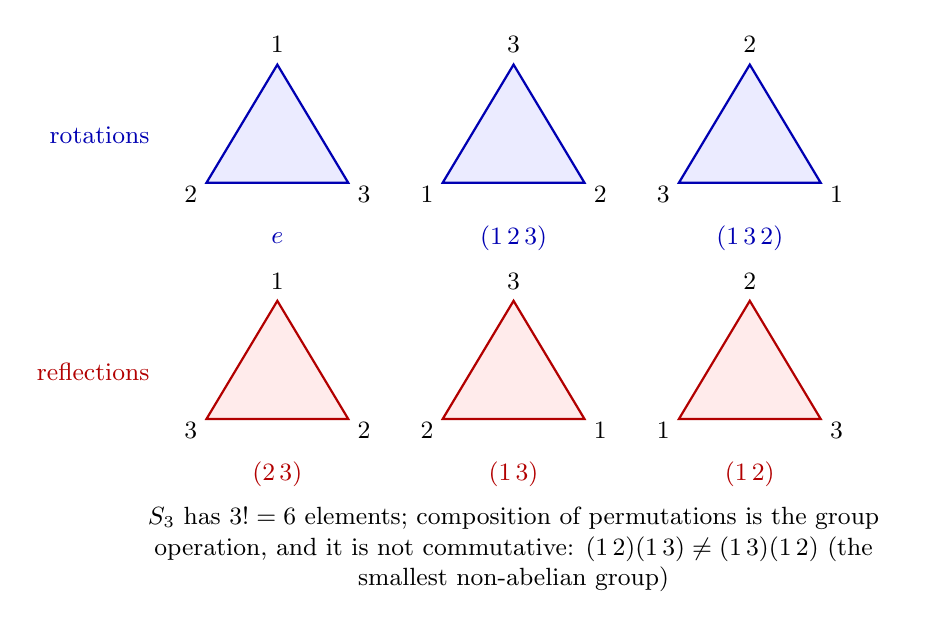
\begin{tikzpicture}[every node/.style={font=\small}]
	\foreach \x/\a/\b/\c/\name in {0/1/2/3/{$e$}, 3/3/1/2/{$(1\,2\,3)$}, 6/2/3/1/{$(1\,3\,2)$}, 0/1/3/2/{$(2\,3)$}, 3/3/2/1/{$(1\,3)$}, 6/2/1/3/{$(1\,2)$}} {
	}
	\foreach \x/\y/\a/\b/\c/\name/\col in {0/0/1/2/3/{$e$}/blue, 3/0/3/1/2/{$(1\,2\,3)$}/blue, 6/0/2/3/1/{$(1\,3\,2)$}/blue, 0/-3/1/3/2/{$(2\,3)$}/red, 3/-3/3/2/1/{$(1\,3)$}/red, 6/-3/2/1/3/{$(1\,2)$}/red} {
		\draw[\col!70!black, thick, fill=\col!8] (\x,\y+0.9) -- (\x-0.9,\y-0.6) -- (\x+0.9,\y-0.6) -- cycle;
		\node[font=\small] at (\x,\y+1.15) {\a};
		\node[font=\small] at (\x-1.1,\y-0.75) {\b};
		\node[font=\small] at (\x+1.1,\y-0.75) {\c};
		\node[\col!70!black, font=\small] at (\x,\y-1.3) {\name};
	}
	\node[blue!70!black, anchor=east] at (-1.5,0) {rotations};
	\node[red!70!black, anchor=east] at (-1.5,-3) {reflections};
	\node[anchor=north, align=flush center, text width=10cm] at (3,-4.6) {$S_3$ has $3!=6$ elements; composition of permutations is the group operation, and it is not commutative: $(1\,2)(1\,3)\neq(1\,3)(1\,2)$ (the smallest non-abelian group)};
\end{tikzpicture}
\end{document}
